\chapter{Our work}
\label{kap:kap3}

In this chapter, we shall look into our proposed enhancements to the existing
implementations of RRR. We at first propose a new block encoding method.
Then, we show how we can exploit the assumptions about the input sequence to
build a better suited implementation for our underlying data. 

\section{Block encoding}

As we already discussed in section~\ref{section:compressed_bv}, there are to
the best of our knowledge two widely used methods to encode and decode the
blocks in RRR. The main disadvantage of the table decoding method is the big space
overhead that it poses and the inability to reasonably support longer blocks
in practice because of the huge table sizes for bigger block lengths. On the
other hand, the on-the-fly decoding method may be used to support a bigger block size
with the downside being longer encoding and decoding times. We propose a
new method of encoding and decoding the blocks. The main objective of the new method is
to create an alternative to the previous methods that enables use of longer blocks
while not hurting the runtime so significantly.

The main idea behind our solution is to use a divide-and-conquer approach to break
the problem of finding the order of the block $B$ along the class $c$ to finding the order
of the several smaller blocks. This may for example enable us to use the table method to solve the
smaller subproblems. To facilitate our solution, we need to alter the respective order of
the blocks along the same class. We want to note that we also use the number of ones to
identify class of the block. On the other hand, both previous solutions used the lexicographical ordering
for the blocks that shared the same class. In our solution, every block $B$ will be thought
of as two smaller \textit{sub-blocks} of half the size, namely $B_1$ and $B_2$ with $B$ being equal to their
concatenation $B_1\cdot B_2$. We shall at first sort the big block $B$ by the pair $(c_1, c_2)$
where $c_1$ and $c_2$ are the respective classes of the smaller sub-blocks $B_1$ and $B_2$. Only then,
we break the tie by lexicographical order of $B_1$ and $B_2$. Note that the original lexicographical
ordering can be rephrased in the context of sub-blocks as sorting at first by $B_1$ and then by
$B_2$. The example of the new ordering for particular block length and class is shown in
Fig.~\ref{obr:lexicographicalVsUs}.

\begin{figure}
	\centerline{
        \begin{tabular}{l c l}
            Offset  &   Block       & $(c_1, c_2)$\\
        \hline
            \small 0&   \tt 000 011 & \multirow{3}{*}{$(0, 2)$}\\
            \small 1&   \tt 000 101 & \\
            \small 2&   \tt 000 110 & \\
        \hline
            \small 3&   \tt 001 001 & \multirow{5}{*}{$(1, 1)$}\\
            \small 4&   \tt 001 010 &\\
            \small 5&   \tt 001 100 &\\
            \small 6&   \tt 010 001 &\\
            \small 7&   \tt 010 010 &\\
        \end{tabular}
        \hspace{3em}
        \begin{tabular}{l c l}
            \small 8&   \tt 010 100 & \multirow{4}{*}{$(1, 1)$}\\
            \small 9&   \tt 100 001 &\\
            \small 10&  \tt 100 010 &\\
            \small 11&  \tt 100 100 & \\
        \hline
            \small 12&  \tt 011 000 & \multirow{3}{*}{$(2, 0)$}\\
            \small 13&  \tt 101 000 &\\
            \small 14&  \tt 110 000 &\\
        \end{tabular}
	}
	\caption[TODO]{
        Example of the new ordering for the block length $b=6$ and class $c=2$.
        Every block is divided into two sub-blocks of size 3. Note the differences to the
        lexicographical ordering. Block {\tt 011 000} on offset 12 is preceded by lexicographicaly
        greater blocks {\tt 100 001}, {\tt 100 010} and {\tt 100 100} as it has bigger number of ones
        in the first sub-block.
    }
	\label{obr:lexicographicalVsUs}
\end{figure}

We shall now demonstrate how we use this new ordering and that it is convenient to encode and
decode block in a divide and conquer manner.

\paragraph{Encoding}

Before providing the general encoding strategy, we shall demonstrate the encoding on
simple example and then generalize the ideas behind the process. Imagine encoding
block {\tt 100 010}. We may observe that the class of this block is 2 as there are two ones in
the whole block. Obtaining the offset is more complicated. We will proceed by enumerating the
number of blocks preceding {\tt 100 010} in the class $c=2$. We divide the blocks preceding
{\tt 100 010} along its class into 3 categories:

\begin{itemize}
    \item Blocks with smaller number of ones in the first sub-block.
    (There are 3 such blocks -- those beginning with {\tt 000}.)
    \item Blocks with same number of ones in the first sub-block, but smaller first sub-block.
    (There are 6 blocks with this property -- those beginning with {\tt 010} or {\tt 001}.)
    \item Blocks with same first sub-block, but smaller second sub-block.
    (There is 1 such block, namely {\tt 100 001}.)
\end{itemize}

Summing up, we get that there are 10 blocks preceding {\tt 100 010} so it has the offset $o$
equal to 10 as we index from 0. Together with its class, we would encode this block as a pair
$(2, 10)$.

In general, consider a block $B$ of length $b$. The first step is to obtain
$c$ -- the class of the block. This can be done by counting ones in $B$, so we
get that $$c=\#_1(B).$$ To obtain the sequence number $o$ of $B$, we shall
count the number of blocks preceding $B$ along the class $c$. As we mentioned,
there are 3 types of blocks preceding $B$:

\begin{enumerate}
    \item Blocks with the first sub-block having smaller class than $B_1$.
    \label{chapter3:encoding:1}
    \item Blocks with the first sub-block being of the same class as is $B_1$
    but with smaller first sub-block. \label{chapter3:encoding:2}
    \item Blocks with the same first sub-block but smaller second sub-block.
    \label{chapter3:encoding:3}
\end{enumerate}

Formalizing this, we shall write $B\prec_X B'$ if blocks $B$ and $B'$ are of
the same length and class and at the same time $B$ precedes $B'$ in ordering $X$.
We write $B\prec_{\Lex} B'$ if $B$ preceeds $B'$ in lexicographical
ordering. To formally define our new proposed ordering $P$, we shall write that
\begin{align*}
    B\prec_P B' \iff
    &[\#_1(B_1) < \#_1(B_1')] \\
    &\lor [(\#_1(B_1) = \#_1(B_1')) \land B_1 \prec_{\Lex} B_1']\\
    &\lor [B_1 = B_1' \land B_2 \prec_{\Lex} B_2']
\end{align*}
where $B=B_1B_2$ and $B'=B_1'B_2'$.

The number of blocks in group~\ref{chapter3:encoding:1} is equal to
$$\sum_{i=0}^{c_1-1} {15\choose i} {15\choose c-i}$$ where $i$ denotes the number
of ones in the first block. Product of term ${15\choose i}$ and ${15\choose c-i}$
denotes the number of blocks with $i$-ones in the first sub-block and the rest
$c-i$ ones in the second sub-block.

The number of blocks in group~\ref{chapter3:encoding:2} is equal to the number of blocks that
share classes of sub-blocks but are smaller than $B$. Number of these blocks is $o_1\times {15\choose c_1}$.
The number of blocks in group~\ref{chapter3:encoding:3} is equal to the number of blocks smaller 
than $B_2$. This is identical to the offset of second sub-block -- $o_2$. Note, that to obtain the
offset of $B$ we need the encoding of the sub-blocks $B_1$ and $B_2$. These are two pairs of numbers
$(c_1, o_1)$ and $(c_2, o_2)$ that can be computed using the on-the-fly encoding or more conveniently,
if the block size is small enough by table encoding.

\paragraph{Decoding}

Decoding is a process of obtaining blocks bit representation $B$ from the encoded
representation $(c, o)$. We would like to reuse the sub-routines for the blocks
of size $b/2$. However, to use these we need to find the classes and offsets of
the smaller sub-blocks. Namely, we need to find what the pairs $(c_1, o_1)$ and
$(c_2, o_2)$ are. This will be a 3 step process. It is easy to observe that $c_1 + c_2 = c$.
All the possible blocks along the class $c$ are primarily sorted by pair $(c_1, c_2)$
that we shall call the class pair. If we know what is the number of blocks along the class $c$
that have the class pair $(c_1, c_2)$ equal to $(0, c), (1, c-1), \ldots , (c, 0)$, we can search
using the offset in which of these groups our block is located. This gives us classes of the sub-blocks
$c_1$ and $c_2$. When we obtain these two, we shall proceed to the second step. Between all the blocks
that have the same $c_1$ and $c_2$, we would like to find $o'$-th along them where the new offset $o'$
is given by subtracting the number of blocks with the smaller class pairs $(c_1, c_2)$, from the offset
$o$. There are ${b/2 \choose c_1}$ and ${b/2 \choose c_2}$ ways how the first and second block may look
respectively. As all the combinations of first and second sub-block are possible, we want to identify
$o'$-th block along the ${b/2 \choose c_1}\cdot {b/2 \choose c_2}$ blocks. Blocks are sorted primarily
by the first sub-block and then by the second sub-block. This means, that the ordered sequence of
the blocks within the class pair $(c_1, c_2)$ will be just all the possible ${b/2 \choose c_2}$
second sub-blocks repeating cyclically, every time with the different, yet increasing
first sub-block. Furthermore, this cycle of ${b/2 \choose c_2}$ sub-blocks will repeat
${b/2 \choose c_1}$ times (once for each possible first sub-block). Using $o'$ we can easily
find the order of the first and second sub-block. We just need to know how many cycles of length
${b/2 \choose c_2}$ happened until $o'$ and what is the offset of the second sub-block at which
the current cycle is on position $o'$. This is straightforward to compute.

% TODO: sem dopisat ako to presne vypocitat
% TODO: nasledujuci example este mozno skryva nejake off by one

We shall again present this process on an example and decode the block from the previous
encoding example {\tt 100 010} encoded as $(2, 10)$. To obtain the number of ones in
the first sub-block only from the offset of the block, we can look into the table and
see that there are 3 blocks with zero ones in the first sub-block. As the offset of our
block is ten, we need to look for this block between blocks with more than 0 ones. There
are 9 blocks with one 1 in the first sub-block. As $3+9$ is bigger than 10, we discovered
that the number of ones in the first block is 1 and it follows that the number of ones in
the second sub-block is
also 1 as we know the total number of ones in the block. There are 9 blocks with
this exact same property, the smallest one being {\tt 001 001} and the largest one
{\tt 100 100}. We had successfully narrowed our search into these 9 blocks and can now
focus on identifying what is the offset of the first and second sub-block. There are
${3 \choose 1} = 3$ possibilities (namely {\tt 001}, {\tt 010}, {\tt 100}) how the first
and also the second sub-block may look. Blocks are sorted according
to the first sub-block and then second sub-block. The cycle through
the sub-blocks will be of length 3 (number of possible second sub-blocks) and will repeat
3 times (number of possible first sub-blocks). Along these ordering of 9 blocks we are
looking for the 7th. From this, we know that the block, we are looking for contains a
first sub-block, that is along all the blocks of size 3 and class 1, third in the ordering.
So to find the first sub-block, we reuse the solution based on the lexicographical ordering
and ask it to decode pair $(1, 2)$ that gives us the first sub-block {\tt 100}. Obtaining
the second sub-block is not that hard. So far, we focused how many times the first sub-block
changes up to the 7th position. Now, we turn our attention on which second sub-block the cycle
ends. We know that every 3rd iteration, the second sub-block starts, where it began.

\paragraph{Extending block size}

Our newly proposed method can be used to obtain the encoding and decoding scheme for block size $2b$
using just a scheme for the block size of $b$. As we already mentioned in
subsection~\ref{subsection:block_size}, most of the implementations of RRR choose the block size of
form $2^k-1$ as the number of possibilities for the value of class is a power of two and
its representation fits exactly into $k$ bits. This is not very convenient for us as combining two
solutions of size $2^k-1$ together gives us only solution for block size $2(2^k-1)$ which is one bit
short of a practically desired size $2^{k+1}-1$. To overcome this, we need to extend the block by one bit.
To do this, we shall once again alter the order of the blocks along the same class. Let us now look on
an example of how we order blocks of length 5 and class 3. There will be two types of blocks
in this class. Ones of the form {\tt 0xxxx} and the rest of the form {\tt 1xxxx}. There are
${4\choose 3}$ ways how to distribute 3 ones along the four places so there will be exactly
4 blocks starting with 0 and ${4\choose 2}$ blocks starting with one. Blocks starting with
zero will continue with all the possible blocks of length 4 and class 3. These blocks could
come in any valid ordering but we can already use our newly devised ordering $P$.
The complete order of the blocks in this example appears in Fig.~\ref{obr:bitExtension}.
\begin{figure}
	\centerline{
        \begin{tabular}{l c}
            Offset  &   Block      \\
        \hline
            \small 0&   \tt 0 0111 \\
            \small 1&   \tt 0 1011 \\
            \small 2&   \tt 0 1101 \\
            \small 3&   \tt 0 1110 \\
        \end{tabular}
        \hspace{4em}
        \begin{tabular}{l c}
            \small 4&   \tt 1 0011 \\
            \small 5&   \tt 1 0101 \\
            \small 6&   \tt 1 0110 \\
            \small 7&   \tt 1 1001 \\
            \small 8&   \tt 1 1010 \\
            \small 9&   \tt 1 1100 \\
        \end{tabular}
	}
	\caption[TODO]{
        Example of bit extension of block length 4 to length 5. Table shows the
        order of blocks along the class $c=3$. These are primarily sorted
        by the first expansion bit. Blocks with the same value of expansion
        bit are sorted according to the method we introduces previously.
    }
	\label{obr:bitExtension}
\end{figure}

We shall call this technique \textit{bit extending} technique. The fact that this
ordering can be encoded and decoded easily is based on the observation that this technique
is just a generalization of our newly devised technique. Up to this point, we combined
scheme for the block size $b$ to obtain solution for block size $2b$. Combining method
for block size $b_1$ with method for block size $b_2$ yields the block size $b_1+b_2$
but we may use the same arguments and ideas for encoding and decoding as we already presented. 

\section{Hybrid encoding}

% TODO: pridat viac kontextu, preco sa zaoberame percentami jednotiek
% TODO: ukazat ze vacsie b je lepsie

The main part of the space-saving aspect of RRR happens because of the way how blocks are stored.
If we have a block of length $b$, then storing it in a raw bit representation takes $b$ bits.
The number of bits used by compressed form depends heavily on the blocks class. If the block
has class $c$, then compressed representation uses $\ceil{\log_2 (b+1)}$ bits to store the
class and $\ceil{\log_2{b\choose c}}$ to store the offset. In Fig.~\ref{obr:rrrSpaceSavings}
we may observe for different block sizes, how the space saved per block depends on the blocks
class. We may observe that RRR saves most of the memory on very sparse or very dense blocks.
We would like to exploit these situations, when the number of ones/zeroes is very low. Thus,
we at first analyze what is the probability distribution of the block classes in a sequence
containing some fixed number of ones distributed randomly. Let us consider a randomly generated
bit sequence $B$ of length $n$ containing $p\%$ of ones.

\begin{figure}
	\centerline{
		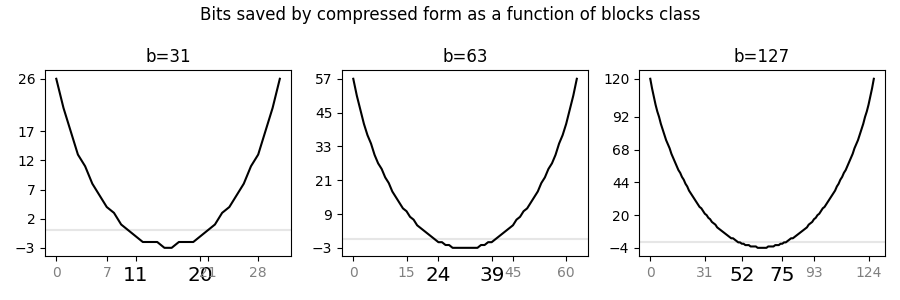
\includegraphics[width=\textwidth]{images/rrr_space_savings}
	}
	\caption[TODO]{Individual graphs present for different block sizes (31, 63, 127), 
    the space saved by using the compressed block representation. We can observe how
    the number of saved bits is dependent on the blocks class. Black numbers on the $x$-axis
    are denoting start and end of the interval where compressed version is worse
    in space usage (negative space saved).
	}
    % can be found on https://github.com/Aj0SK/master-thesis/blob/main/text/images/rrr_space_savings.png
	\label{obr:rrrSpaceSavings}
\end{figure}

If we consider a block size $b$ then the random variable $X$ denoting number of ones in
block follows a binomial distribution $$X \sim Bin(b,p).$$ As we may observe in
Fig.~\ref{obr:hybridEncodingDistribution}, the probability of blocks
containing a lot of ones decreases exponentially in a sequence containing only 5\% of ones.
Even in very long sequences, these blocks will occur very rarely. This gaved us
opportunity to a solution that we call \textit{hybrid encoding}.

\begin{figure}
	\centerline{
		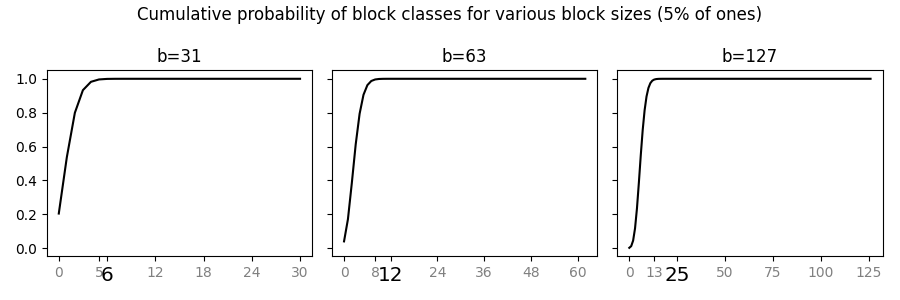
\includegraphics[width=\textwidth]{images/hybrid_encoding_motivation}
	}
	\caption[TODO]{On these 3 graphs, we can see the cumulative distribution
    of blocks classes for the block sizes 31, 63, 127. The frequency of ones is
    fixed to 5\%. Note the marked classes on the $x$-axis. Numbers 6, 12 and
    25 mark the place up to which 99\% of probability distribution lies for
    the block sizes 31, 63 and 127 respectively.
	}
    % Can be found on https://github.com/Aj0SK/master-thesis/blob/main/text/images/hybrid_encoding_motivation.png
	\label{obr:hybridEncodingDistribution}
\end{figure}

The hybrid encoding uses a property that in some sequences blocks with high number
of ones are very rare. Encoding these blocks is not that beneficial as their
compressed representation may take even more bits than the original raw
representation. Storing the whole block may waste space if the number of
ones is big but there are not many possibilities how the block may look.
Although we waste some space by this approach from time to time (for every
block that is densely packed with ones), we can save some small
amount of space by decreasing the number of bits used to store the classes.
The main idea of hybrid encoding is that every block with its
class bigger than some threshold will have its class set to this threshold
and this will mean that the block is stored using full $b$ bits instead of
$\ceil{\log_2{b\choose c_i}}$ bits. When we choose a $c_k$ as a value for cut off
then blocks with class bigger or equal to $c_k$ will not be encoded but just
copied with the class set to $c_k$ no matter what is the number of ones in them.
Note that the class of the block
is a number from 0 up to $b$. To possibly save some space on the bit representation
of the blocks class, we need to choose $c_k$ such that $\ceil{\log_2(c_k+1)} < \ceil{\log_2(b+1)}$.
We shall now compare these two representations and the theoretical space savings that
can be obtained. Let $n$ be a length of the sequence, $b$ the block size and $C_i$
number of blocks with class $i$. To simplify the calculations, we shall assume that $b+1$
as well as $c_k$ is a power of 2 and $n$ is divisible by $b$, also we shall
denote logarithm with base 2 $\lg x$. Using this notation, first representation is
consuming $$(n/b)\lg (b+1) + \sum_{i=0}^{b} C_i\ceil{\lg {b\choose i}}$$
bits of space with the first and second term being the number of bits that
is used by the classes and offsets respectively. The second representation
with the cutoff $c_k$ shall consume $$(n/b)\lg (c_k+1) + \sum_{i=0}^{c_k-1}C_i\ceil{\lg {b\choose i}} + \sum_{i=c_k}^{b}C_i b$$
bits of space. We would like to find out what is the expected space that we save
using the hybrid encoding. We start by simplifying the expected value of the
difference of these representations:
% My mathematical guesswork
\begin{align}
E[space] &= E\left[(n/b)(\lg(b+1)-\lg(c_k+1)) + \sum_{i=c_k}^{i\leq b}\ceil{C_i}\cdot \left(\ceil{{b\choose i}} - b\right)\right] \nonumber\\
&=(n/b)(\lg(b+1)-\lg(c_k+1)) + \sum_{i=c_k}^{i\leq b}E\left[\ceil{C_i}\cdot \left(\ceil{{b\choose i}} - b\right)\right] \nonumber\\
&=(n/b)(\lg(b+1)-\lg(c_k+1)) + \sum_{i=c_k}^{i\leq b}\ceil{E\left[C_i\right]}\cdot \left(\ceil{{b\choose i}} - b\right) \nonumber\\
E[C_i] &= (n/b)\cdot {b\choose i}\cdot p^i\cdot (1-p)^{b-i} \label{eq:hybrid_encoding_expected_c_i}
\end{align}

Here we mainly used the linearity of the expected value. To compute the expected value of
$C_i$ we used the fact, that number of blocks of a certain class follows binomial
distribution. We know that in the bit sequence, there is $p\%$ of ones. There is $n/b$ blocks
and each has probability ${b\choose i}p^i(1-p)^{b-i}$ for being of class $i$. This probability
is independent from the previous blocks and as we are interested in total number of blocks with
this class, it follows that $C_i$ follows binomial distribution. As
$$C_i \sim Bin(n/b, {b\choose i}p^i(1-p)^{b-i})$$ it follows that the expected value is equal to
\ref{eq:hybrid_encoding_expected_c_i}.

We present the expected space saved by hybrid implementation for some chosen values of
$p, b$ and $c_k$ in Fig.~\ref{obr:hybridEncodingTheoretical}.
% TODO: space saved should be used, need to regenerate to 1-x
\begin{figure}
	\centerline{
        \begin{tabular}{l c c c}
            $p$                 & $b$   &   $c_k$   &  {\tt used space}\\
        \hline
            \multirow{7}{*}{5}  &   31  &   7       &   0.83\\
                                &   31  &   15      &   0.91\\
                                &   63  &   15      &   0.91\\
                                &   63  &   31      &   0.95\\
                                &   127 &   7       &   1.86\\
                                &   127 &   15      &   0.93\\
                                &   127 &   63      &   0.98\\
        \end{tabular}
        \hspace{4em}
        \begin{tabular}{l c c c}
                                &       &           &       \\
            \multirow{7}{*}{10} &   31  &   7       &   0.90\\
                                &   31  &   15      &   0.94\\
                                &   63  &   15      &   0.94\\
                                &   63  &   31      &   0.97\\
                                &   127 &   7       &   2.03\\
                                &   127 &   15      &   1.22\\
                                &   127 &   63      &   0.99\\
        \end{tabular}
        %\hspace{4em}
	}
	\caption[TODO]{
        We may observe the ratio of expected space used by the hybrid implementation to space used by our
        standard RRR implementation for varios percentage of ones in the text -- $p$ as well as for
        different block size -- $b$ and cutoff value -- $c_k$. 
    }
	\label{obr:hybridEncodingTheoretical}
\end{figure}
We may observe, that for some choices of cut-off, we may expect to save rougly 10-17\%
of space compared to the original method. On top of this, hybrid encoding approach has a potential
to be of the same or even better performance as it is easier to decode the blocks
saved in the raw form. However, we should note that hybrid encoding is based on the expectation
that the number of these blocks is low, so the possible speedup may not be very significant.
% some rough numbers from the program:
% https://github.com/Aj0SK/master-thesis/blob/main/code/experiment3/sdsl_theoretical_stat.py
% n, b, c_k, p     ->  classic vs hybrid and hybrid/classic
% For 100000, 31, 7, 0.05 the result is 37591 vs 31161 ... rate 0.83
% For 100000, 31, 15, 0.05 the result is 37591 vs 34365 ... rate 0.91
% For 100000, 63, 7, 0.05 the result is 33727 vs 30904 ... rate 0.92
% For 100000, 63, 15, 0.05 the result is 33727 vs 30553 ... rate 0.91
% For 100000, 63, 31, 0.05 the result is 33727 vs 32140 ... rate 0.95
% For 100000, 127, 7, 0.05 the result is 31533 vs 58547 ... rate 1.86
% For 100000, 127, 15, 0.05 the result is 31533 vs 29257 ... rate 0.93
% For 100000, 127, 31, 0.05 the result is 31533 vs 29958 ... rate 0.95
% For 100000, 127, 63, 0.05 the result is 31533 vs 30746 ... rate 0.98
% For 100000, 31, 7, 0.1 the result is 54158 vs 48597 ... rate 0.90
% For 100000, 31, 15, 0.1 the result is 54158 vs 50932 ... rate 0.94
% For 100000, 63, 7, 0.1 the result is 51211 vs 67717 ... rate 1.32
% For 100000, 63, 15, 0.1 the result is 51211 vs 48065 ... rate 0.94
% For 100000, 63, 31, 0.1 the result is 51211 vs 49624 ... rate 0.97
% For 100000, 127, 7, 0.1 the result is 49421 vs 100448 ... rate 2.03
% For 100000, 127, 15, 0.1 the result is 49421 vs 60378 ... rate 1.22
% For 100000, 127, 31, 0.1 the result is 49421 vs 47847 ... rate 0.97
% For 100000, 127, 63, 0.1 the result is 49421 vs 48634 ... rate 0.98
% For 100000, 31, 7, 0.15 the result is 67370 vs 65690 ... rate 0.98
% For 100000, 31, 15, 0.15 the result is 67370 vs 64144 ... rate 0.95
% For 100000, 63, 7, 0.15 the result is 64885 vs 95458 ... rate 1.47
% For 100000, 63, 15, 0.15 the result is 64885 vs 62736 ... rate 0.97
% For 100000, 63, 31, 0.15 the result is 64885 vs 63298 ... rate 0.98
% For 100000, 127, 7, 0.15 the result is 63305 vs 102345 ... rate 1.62
% For 100000, 127, 15, 0.15 the result is 63305 vs 96077 ... rate 1.52
% For 100000, 127, 31, 0.15 the result is 63305 vs 61809 ... rate 0.98
% For 100000, 127, 63, 0.15 the result is 63305 vs 62518 ... rate 0.99
% For 100000, 31, 7, 0.2 the result is 78024 vs 82507 ... rate 1.06
% For 100000, 31, 15, 0.2 the result is 78024 vs 74802 ... rate 0.96
% For 100000, 63, 7, 0.2 the result is 75829 vs 103481 ... rate 1.36
% For 100000, 63, 15, 0.2 the result is 75829 vs 78570 ... rate 1.04
% For 100000, 63, 31, 0.2 the result is 75829 vs 74242 ... rate 0.98
% For 100000, 127, 7, 0.2 the result is 74384 vs 102362 ... rate 1.38
% For 100000, 127, 15, 0.2 the result is 74384 vs 102863 ... rate 1.38
% For 100000, 127, 31, 0.2 the result is 74384 vs 75460 ... rate 1.01
% For 100000, 127, 63, 0.2 the result is 74384 vs 73596 ... rate 0.99
